% !TeX document-id = {8751af90-d4b1-40f9-88be-89e61cd71d0c}
% !TeX TXS-program:compile = txs:///pdflatex/[--shell-escape]
\documentclass[a4paper,11pt]{article}

%\usepackage[style=apa]{biblatex}
\usepackage[style=apa,sortcites=true,sorting=nyt,backend=biber]{biblatex}
\usepackage{amsmath,amsfonts,amssymb, bm}
\usepackage{graphicx,verbatimbox}
\usepackage[colorlinks=true, allcolors=blue]{hyperref}
\usepackage[margin=1in]{geometry}
\usepackage{authblk}
\usepackage{nicefrac}
\usepackage{svg}
\usepackage{booktabs}
\usepackage{makecell} %\thead
\usepackage{array}
\newcolumntype{H}{>{\setbox0=\hbox\bgroup}c<{\egroup}@{}} % hidden column


%opening
\title{Augmenting Predictive Models in Forensic Psychiatry with Cultural Consensus Theory}
\author[1]{Don van den Bergh}
\author[2]{Erwin Schuringa}
\author[1]{Eric-Jan Wagenmakers}
\affil[1]{Department of Psychological Methods, University of Amsterdam}
\affil[2]{Forensic Psychiatric Center Dr. S. van Mesdag}
\date{}

%\usepackage[dvipsnames]{xcolor}
\usepackage{xcolor}
\usepackage{todonotes}

\definecolor{colorDon}{RGB}{205,250,255}
\definecolor{colorEJ} {RGB}{205,255,205}

\newcommand{\DB}[1]{\todo[inline, color=colorDon]{DB: {#1}}}
\newcommand{\DBB}[1]{\todo[color=colorDon]{DB: {#1}}}
\newcommand{\EJ}[1]{\todo[inline, color=colorEJ]{EJ: {#1}}}

\newcommand{\githuburl}{\url{https://github.com/vandenman/CCT-Logistic}}

\graphicspath{{../figures/}{../graphicalmodels/}}

\addbibresource{references.bib}

\newcommand{\fig}{Fig.}


\newcommand{\Irater}{r}
\newcommand{\Iitem}{i}
\newcommand{\Ipatient}{p}
%\newcommand{\Incat}{c}
%\newcommand{\Ilatent}{l}
%\newcommand{\IdiscreteP}{d}
\newcommand{\Icovariate}{c}

\newcommand{\Trater}{\expandafter\MakeUppercase\expandafter{\Irater}}
\newcommand{\Titem}{\expandafter\MakeUppercase\expandafter{\Iitem}}
\newcommand{\Tpatient}{\expandafter\MakeUppercase\expandafter{\Ipatient}}
%\newcommand{\Tncat}{\expandafter\MakeUppercase\expandafter{\Incat}}
%\newcommand{\Tlatent}{\expandafter\MakeUppercase\expandafter{\Ilatent}}
%\newcommand{\TdiscreteP}{\expandafter\MakeUppercase\expandafter{\IdiscreteP}}
\newcommand{\Tcovariate}{\expandafter\MakeUppercase\expandafter{\Icovariate}}

% definitions of variables
\newcommand{\ItemTruth}{\theta}
\newcommand{\ItemDifficulty}{\kappa}
\newcommand{\UnBiasedThreshold}{\gamma}
\newcommand{\Threshold}{\delta}
\newcommand{\RaterScale}{\alpha}
\newcommand{\RaterShift}{\beta}
\newcommand{\RaterCompetence}{\zeta}
\newcommand{\Appraisal}{y}
\newcommand{\Error}{\epsilon}
\newcommand{\FactorScore}{\eta}
\newcommand{\FactorRegression}{\lambda}
%\newcommand{\RaterCovariate}{z}
%\newcommand{\PatientCovariate}{w}
\newcommand{\Covariate}{z}

\newcommand{\CovariateBeta}{\delta}
\newcommand{\ItemCovariateBeta}{\gamma}


% Probability distributions

%\newcommand{\ilogit}[1]{\text{logit}^{-1}\left(#1\right)}
\newcommand{\ilogit}[1]{\begin{revision}F\end{revision}\left(#1\right)}
\newcommand{\logit}[1]{\text{logit}\left(#1\right)}
\newcommand{\dnorm}[2]{\text{Normal}\left(#1,\,#2\right)}
\newcommand{\dnormp}[2]{\text{Normal\textsuperscript{+}}\left(#1,\,#2\right)}
\newcommand{\dgamma}[2]{\text{Gamma}\left(#1,\,#2\right)}
\newcommand{\dgammaMV}[2]{\text{Gamma}\left(\nicefrac{#1^2}{#2},\,\nicefrac{#1}{#2}\right)} % #1 is mean, #2 is variance
\newcommand{\dlognormal}[2]{\ensuremath{\mathrm{LogNormal}\left(#1,\,#2\right)}}
\newcommand{\dlogis}[2]{\text{Logistic}\left(#1,\,#2\right)}
\newcommand{\dlogiss}[3]{\text{Logistic}\left(#1;\,#2,\,#3\right)}

\newcommand{\dinvgamma}[2]{\text{InverseGamma}\left(#1,\,#2\right)}

% math commands
\newcommand{\assignment}{=}
\newcommand{\SE}[1]{\emph{({#1})}}
\newcommand{\code}[1]{\texttt{#1}}

% spaces
\newcommand{\Reals}{\mathbb{R}}
\newcommand{\PositiveReals}{\Reals^+}

% abbreviation Anders & Batchelder (2015)
\newcommand{\AB}{AB}


\begin{document}

\maketitle

\tableofcontents

\begin{abstract}

\end{abstract}

\section{Introduction}
The mental health and forensic risk factors of patients in forensic psychiatric hospitals is regularly monitored with methods such as
Routine Outcome Monitoring \parencite{deBeurs2011ROM}.
A staff member (e.g., a clinician or psychiatrist), henceforth a \emph{rater}, scores a patient on variety of criteria, such as problematic behavior (e.g., hostility) or protective behavior (e.g., coping skills).
These scores are used to track the mental state of patients over time, to measure the effectiveness of treatment, and as a risk indicator for violent outbursts by patients.
% Using these scores raters can monitor the mental state of a patient over time, answer questions about the effectiveness of a treatment, or warn staff members about which patients are at risk for turning violent. 

Typically, multiple raters score each patient on different items.
Standard practice is to average the scores across raters and use the averages to inform decisions.
However, this is suboptimal for multiple reasons \parencite{vandenBergh2020cultural}.
For example, taking the average implies that raters are interchangeable and patients are independent, rather than taking into account raters' bias or patients' offense.
% For example, this implies raters are exchangeable and patients are independent, rather than accounting for raters' biases or patients' criminal offense.

% In a typical data set there are for each patient multiple scores available on different items, given by different raters.
% Standard practice is to average the scores across raters and use those to inform decisions.
% This practice is suboptimal, as it treats raters as exchangeable and analyzes patients independently.

An improvement over averaging the scores is to use Cultural Consensus Theory \parencite[CCT;][]{romney1986culture, batchelder1988test, batchelder2012cultural} to construct an appropriate model for the scores that accounts for the hierarchical structure among patients, raters, and items. 
In previous work, we developed such a model based on the Latent Truth Rater model \parencite[LTM; ][]{Anders2015cultural}, and demonstrated that, in theory, this model predicted better than the average and several machine learning alternatives.
However, due to the lack of an empirical dataset, we could not demonstrate whether the theoretical claims hold up in practice.

% In previous work, we used Cultural Consensus Theory \parencite[CCT;][]{romney1986culture, batchelder1988test, batchelder2012cultural} to develop an appropriate model to analyze such data that accounts for the hierarchical structure among patients, raters, and items \parencite{vandenBergh2020cultural}.

Here, we apply the CCT-based model to data of a Dutch maximum-security forensic psychiatric center and use its inferences to predict whether or not a patient becomes violent.
First, we briefly introduce the LTM model used and discuss two changes made compared to \textcite{vandenBergh2020cultural}.
Afterward, we use the LTM to augment a logistic regression.
We use the augmented model to predict violent outbursts in patients and compare the predictive performance to that of frequently used machine learning models.
We find that our LTM approach outperforms all other methods, albeit by a small margin.
Next, we interpret the fitted model and ...
% The paper is concluded with a discussion on how the data collection could be adjusted to maximize the benefit of our CCT-based approach.
Finally, we discuss some practical limitations of the data set at hand and how future monitoring of patients could be adjusted to maximize the added benefit of our CCT-based approach.


\section{Mesdag Data}
\DB{Edwin, het zou fijn zijn als jij naar deze sectie kan kijken!}
\subsection{Method of collection}
The data were collected in the Dutch maximum-security Forensic Psychiatric Center Dr. S. van Mesdag in the period XXX to XXX.\DBB{April 2010 t/m juli 2016 gok ik gebaseerd op Schuringa et al. 2016.}
The individual records were retrospectively merged into a single data set.

\subsection{IFTE}
The data were collected using a Routine Outcome Monitoring instrument called the the Instrument for Forensic Treatment Evaluation (IFTE).
The IFTE consists of 22 items, of which 14 items are criminogenic need indicators of the Dutch risk assessment instrument HKT-R \parencite{spreen2013handleiding}, five items were designed in consultation with psychologists and psychiatrists, and three items are based on the Atascadero Skills Profile \parencite{vess2001development}.
The 22 items can be grouped into three factors, Protective behaviors, Problematic behaviors, and Resocialization Skills.
The individual items are shown in \autoref{tb:IFTE_items}.
All items are scored on a 18 point scale.

\subsection{Covariates}
In addition to the IFTE, several other background variables about the patients are considered for predicting violent behavior.
These are age (0-30, 31-40, 41-50, or 55+), treatment duration (0-2 years, 2-4 years, 4-6 years, or 6+ years), diagnosis (Autism spectrum disorder, Personality disorder, Personality disorder B, Schizophrenia or other psychotic disorders, As 1 overig), offence (Manslaughter, Aggravated assault, Murder, Arson, Violent property crime, Moderately violent property crime, Sexual offence), violent behavior before measurement 1, and violent behavior in between measurements 1 and 2.
\DB{Check de juiste engelse vertalingen.}


\subsection{Descriptives}
\autoref{fig:descriptives_scores_hist} shows a histogram of the raw scores across all IFTE items, raters, and patients.
It is clear that some scores are given more often than others, such as 1, 2, 6, 10, and 14.
Furthermore, it appears that, with the exception of 1, even scores are given more often than odd scores.


\begin{figure}[!ht]
	\centering
	\includesvg[width=\textwidth]{descriptives_scores}
	\caption{Histogram of observed scores across all patients, items, raters, and time points.}
	\label{fig:descriptives_scores_hist}
\end{figure}

Not all raters rated every patient, in contrast, \autoref{fig:descriptives_raters_by_patients} shows that the rater by patient matrix is rather sparse.
\begin{figure}[!ht]
	\centering
	\includesvg[width=\textwidth]{descriptives_raters_by_patients}
	\caption{Heatmap of observed scores of rater ($x$-axis) against patients ($y$-axis).}
	\label{fig:descriptives_raters_by_patients}
\end{figure}

\section{Cultural Consensus Theory}

Cultural Consensus Theory, sometimes called ``test theory without an answer key'' \parencite{batchelder1988test}, is a method to discover the ''true answer`` for items from the consensus among the responses.
For example, suppose a patient is scored by multiple raters on aggressiveness.
Multiple scores are obtained that need to be aggregated to arrive at a single score for this patient.
The naive solution is to average these scores.
However, as shown in \autoref{fig:misFitMean} averaging may lead to severely biased estimates.
\begin{figure}[!ht]
	\centering
	\includesvg[width=\textwidth]{misfitMean}
	\caption{True item scores (x-axis) versus the sample mean across raters (y-axis).}
	\label{fig:misFitMean}
\end{figure}
The average score disregards all additional information that is available.
It ignores the individual differences between raters, for example, this assumes that all psychiatrists score aggressiveness in the same way, and it ignores group differences among raters, for example, there is no difference in scores by psychiatrists as opposed to clinicians, or other staff member.
In addition, the average ignores any additional information about the patient at hand, such as offence and diagnosis.

Cultural consensus theory provides a model-based framework for pooling information from multiple raters to form a consensus \parencite{anders2014cultural}.
There exist a variety of CCT models, each applicable to different types of data.
For example, the General Condorcet model \parencite{Batchelder1986statistical} applies to dichotomous data, the Continuous Response model \parencite{anders2014cultural} is suited for continuous data, and the Latent Truth Rater model \parencite{Anders2015cultural} is suited for ordinal data.
As the ratings on the are ordinal, we use the Latent Truth Rater model to analyze the Mesdag data.

\subsection{The Latent Truth Rater Model}
The Latent Truth Rater Model (LTM) is a CCT model for ordinal data \parencite{Anders2015cultural}.
Previously, we extended the LTM to handle data from multiple patients \parencite{vandenBergh2020cultural} and \autoref{model:LTM_p} shows the LTM for multiple patients.
\begin{figure}[!ht]
	\begin{minipage}{0.55\textwidth}
		\centering
		\includegraphics[width=\textwidth, page=7]{graphicalmodels.pdf}
	\end{minipage}\hfill
	\begin{minipage}{0.45\textwidth}
		{\normalsize
			\begin{align*}
			\oneScore &\assignment
			\begin{cases}
			1		&\hspace{-.3cm} \text{if } \oneAppraisal \leq \Threshold_{\Irater 1} \\
			\Incat	&\hspace{-.3cm} \text{if } \Threshold_{\Irater, \Incat-1} < \oneAppraisal \leq \Threshold_{\Irater\Incat} \\
			\Tncat	&\hspace{-.3cm} \text{if } \oneAppraisal > \Threshold_{\Irater, \Tncat-1}
			\end{cases}\\
			\oneAppraisal &\sim \dlogis{\ItemTruth_{\Ipatient\Iitem}}{\nicefrac{\ItemDifficulty_\Iitem}{\RaterCompetence_\Irater}} \\
			\Threshold_{\Irater\Incat} &\sim \dnorm{0}{1}\\
			\ItemTruth_{\Ipatient\Iitem}        &\sim \dnorm{\mu_\ItemTruth}{\sigma_\ItemTruth^2}\\
			\ItemDifficulty_\Iitem   &\sim \dgammaMV{\mu_\ItemDifficulty}{\sigma_\ItemDifficulty^2} \\
			\RaterCompetence_\Irater &\sim \dgammaMV{\mu_{\RaterCompetence_\Irater}}{\sigma_{\RaterCompetence_\Irater}^2} \\
			\end{align*}
		}%
	\end{minipage}
	\caption{%
		Graphical model of the Latent Truth Rater Model for multiple patients.
		Note that the thresholds $\bm{\Threshold}_\Irater$ are constrained to be ordered, that is, for all raters we have $\Threshold_{\Irater 1} \leq \dots \leq \Threshold_{\Irater \Incat} \leq \dots \leq \Threshold_{\Irater,\Tncat-1}$.
	}
	\label{model:LTM_p}
\end{figure}

Here, $\oneScore$ is the observed score given to patient $\Ipatient$ on item $\Iitem$ by rater $\Irater$.
This score is assumed to be deterministically generated from a continuous latent appraisal $\Appraisal_{\Ipatient\Iitem\Irater}$ that is discretized to an ordinal scale by the thresholds $\Threshold_{\Irater\Incat}$.
In particular, we have that
\begin{align*}
\oneScore =
\left\{\begin{array}{ll}
1		& \text{if }  \Appraisal_{\Ipatient\Iitem\Irater} \leq \Threshold_{\Irater 1} \\[4pt]
\Incat	& \text{if }  \Threshold_{\Irater, \Incat - 1} < \Appraisal_{\Ipatient\Iitem\Irater} \leq \Threshold_{\Irater\Incat} \\[4pt]
\Tncat	& \text{if }  \Appraisal_{\Ipatient\Iitem\Irater} > \Threshold_{\Irater,\Tncat-1}
\end{array} \right.
\end{align*}
Since the appraisal score is latent, the deterministic function above implies the following probabilistic model over the observed scores:
\begin{align*}
P(\oneScore\mid \oneAppraisal,\bm{\Threshold}_{\Irater}) =
\left\{\begin{array}{ll}
1 - \cdf{\Appraisal_{\Ipatient\Iitem\Irater} - \Threshold_{\Irater 1}}         & \text{if } \oneScore = 1, \\[4pt]
\cdf{\oneAppraisal - \Threshold_{\Irater,\Incat-1}} -
\cdf{\oneAppraisal - \Threshold_{\Irater\Incat}}         & \text{if } 1 < \oneScore < \Tncat,\\[4pt]
\cdf{\oneAppraisal - \Threshold_{\Irater,\Tncat-1}}       & \text{if } \oneScore = \Tncat.
\end{array} \right.
\end{align*}
where $\cdf{}$ is the logistic cumulative distribution function.\footnote{%
	Note that this choice is arbitrary and that it is possibly to use any continuous cumulative distribution function.
}

Next, we explain how the latent appraisals and thresholds come about.
The appraisals are draws from a logistic distribution with location $\ItemTruth_{\Ipatient\Iitem}$, the true score for patient $\Ipatient$ on item $\Iitem$. The scale of the logistic distribution is the ratio of the item difficulty $\ItemDifficulty_\Iitem$ to the rater competence $\RaterCompetence_\Irater$.
A higher item difficulty means that the appraisals are more noisy, which leads to a more dispersed probability distribution over possible scores.
Conversely, a higher rater competence means that the appraisals are less noisy, which leads to a more concentrated distribution over the outcomes.
There are $\Tncat - 1$ ordered thresholds for each rater, which are assigned a standard normal prior for identification purposes.

There are two differences in the model specification above compared to our previous work \parencite{vandenBergh2020cultural}.
%We made two changes to the model, because when simulating data with similar characteristics as the Mesdag data, as
First, we previously modeled the thresholds using two rater specific parameters.
However, in simulations we noticed that these two parameters provide too little flexibility when the ordinal scale consists of 18 categories and has a multimodal distribution (see \autoref{fig:descriptives_scores_hist}), as in the Mesdag data.
Therefore we decided to model the thresholds individually.
This complicates interpreting the differences between the thresholds across raters, however, that is also not the goal of this paper.
Second, we previously allowed the item difficulty parameter to vary across patients, which captures that some items may be more difficulty or easy to assess for some patients (e.g., some patients may cooperate more than others).
This parameter is mainly informed by the number or raters and there needs to be a sufficient amount of raters that score each patient for a reliable estimate.
However, when simulating data with a ratio of raters to patients similar to that in the data at hand that we noticed that there are simply too few observations to reliably estimate the deviations in item difficulty across patients.
Therefore, we only vary item difficulty across items and not across patients. 
% \DB{We could also look at a patient specific ``cooperativeness'' parameter. Rather than doing $\ItemDifficulty_{\Ipatient\Iitem}$, which introduces $\Tpatient\times\Titem$ parameters, the logistic scale would become $\frac{\ItemDifficulty_\Iitem}{\RaterCompetence_\Irater \times\text{Cooperativeness}_\Ipatient}$. This introduces an additional $\Tpatient$ parameters.}


%$\Appraisal_{\Ipatient\Iitem\Irater} \leq \Threshold_{\Irater1}$ implies that $x_{\Ipatient\Iitem\Irater} = 1$, $\Threshold_{\Irater, \Incat - 1} < \Appraisal_{\Ipatient\Iitem\Irater} \leq \Threshold_{\Irater\Incat}$ implies that $x_{\Ipatient\Iitem\Irater} = \Incat$, and $\Appraisal_{\Ipatient\Iitem\Irater} > \Threshold_{\Irater\Tncat}$ implies that $x_{\Ipatient\Iitem\Irater} = \Tncat$.
%
%  that distributed with mean $\mu_{\Ipatient\Iitem\Irater}$ and standard deviation $\sigma_{\Iitem\Irater}$.
%
%
%Compared to our previous work, we made a few adjustments to make the model more suited for analyzing the data at hand.
%First, we removed
%
%
%Previously we modeled the thresholds using two rater specific parameters. However, during simulations we noticed that this is too restrictive when the ordinal scale consists of 18 categories, as in the data example at hand.


\subsection{Augmenting Logistic Regression with the LTM}
In a next step, we use logistic regression for to predict violent behavior, where we use the results from the LTM as additional predictors.
We do so in a fully Bayesian approach, that is, we constructed a joint model for the violent behavior and then patient ratings.%
\footnote{%
An alternative is to fit the LTM separately and then use e.g., the posterior means in a second step in a logistic regression.
While this would be more computationally efficient, it would also ignore the uncertainty in the analysis of the patient ratings.
}
\autoref{model:Logistic_LTM} shows a graphical model of the logistic regression combined with the LTM.
The latent truth for each patient on each item is seen as a covariate in the logistic regression model.

\subsection{Implementation}
We estimated the parameters of the LTM and the combined LTM -- Logistic regression using a Bayesian approach.
To explore the posterior distributions of the model parameters we used Stan \parencite{CarpenterEtAl2017Stan}. 
Rather than Markov chain Monte Carlo (MCMC) we used variational inference, as variational inference was computationally fast while providing similar results in terms of parameter retrieval and model predictions \parencite{kucukelbir2017automatic}. 
All analyses were done using R \parencite{R} and Stan models were run using the R package \code{cmdstanr} \parencite{cmdstanr}. 
Code for the analyses is available in the online appendix at \githuburl{}.

%with a logistic regression
%In our application we are not directly interested in the results of the LTM, but rather, we wish to predict violent behavior
%The CRM applies an information pooling strategy. Here, we use the results from the CRM, specifically the item truths for each patient, to augment prediction of aggressiveness.

\begin{figure}[!ht]
%	\begin{minipage}{0.5\textwidth}
		\centering
		\includegraphics[width=\textwidth, page=8]{graphicalmodels.pdf}
%	\end{minipage}\hfill
%	\begin{minipage}{0.5\textwidth}
%		{\normalsize
%			\begin{align*}
%			x_{\Ipatient\Iitem\Irater}      &\sim \dnorm{\mu_{\Ipatient\Iitem\Irater}}{\sigma^2_{\Ipatient\Iitem\Irater}} \\
%			\mu_{\Ipatient\Iitem\Irater}    &\assignment \RaterScale_\Irater \ItemTruth_{\Ipatient\Iitem} + \RaterShift_\Irater  \\
%			\sigma_{\Iitem\Irater} 			&\assignment \RaterCompetence_\Irater \ItemDifficulty_\Iitem\\
%			\ItemTruth_{\Ipatient\Iitem}	&\sim \dnorm{\mu_\ItemTruth}{\sigma^2_\ItemTruth}\\
%			\log \ItemDifficulty_\Iitem 	&\sim \dnorm{\mu_\ItemDifficulty}{\sigma^2_\ItemDifficulty}\\
%			\log \RaterScale_\Irater     	&\sim \dnorm{\mu_\RaterScale}{\sigma^2_\RaterScale}\\
%			\RaterShift_\Irater	   			&\sim \dnorm{\mu_\RaterShift}{\sigma^2_\RaterShift}\\
%			\log \RaterCompetence_\Irater	&\sim \dnorm{\mu_\RaterCompetence}{\sigma^2_\RaterCompetence}\\
%			\end{align*}
%		}%
%	\end{minipage}
	\caption{Graphical model of Logistic Regression Augmented with the Latent Truth Rater Model.}
	\label{model:Logistic_LTM}
\end{figure}

% \iffalse
% \subsection{Simulation Study}

% Before analyzing the data with the LTM, it is typically a good idea to run a simulation study to

% \subsubsection{Do we actually want to report this?}

% \subsubsection{Fit of the LTM}
% \fi

\section{Predictive Performance}

Here we compare the predictive performance of the Logistic regression augmented with the LTM (LR-LTM) to several reasonable alternatives and three baseline models.
As a first baseline model we use an intercept only logistic regression (LR-Intercept), which quantifies if we can outperform the base-prevalence of violence.
The second baseline model we use is a logistic regression model with all covariates but not the IFTE items (LR-No IFTE).
% TODO: wat is de toegevoegde waarde van model 3 bovenop model 2?
As a third baseline model, we use an logistic regression model with only prior violence as predictors (LR-Violence).
As more reasonable alternatives, we consider logistic regression (LR), random forest, and boosted regression trees (GBM) which have access to all history of violence, patient covariates, and IFTE scores.
These four alternative have in common that they are designed for purely rectangular data.
That is, each row of the data set contains one outcome (aggressive behavior or not) and a number of predictors.
However, the raw data of the IFTE contains repeated observations, since patients were rated multiple times by different raters.
To accommodate this we average across different raters to obtain a single scores for each item and time point.
By comparing these models we aim to answer the following three questions: (1) Can predictive models outperform the base-prevalence of violent behavior? (2) Do models with the IFTE scores perform better than the baseline models without? (3) Does the LR-LTM perform better than the models that naively average across raters?

To examine predictive performance we used 10-fold stratified cross validation.
Each fold consisted of 8 nonviolent observations and 2 or 3 violent observations.
% For every fold, the data were split into a training set (80\%, $N = 84$) and a test set (20\%, $N = 20$).
% The models were fit on the training set and made predictions for the test set.
To quantify model performance, we used two metrics, prediction accuracy and the Brier score.
Prediction accuracy is defined as the fraction of correct predictions.
We converted model probabilities for violent or non-violent behavior into binary predictions by comparing with 0.5. In other words, if a model prediction for observation $i$, $\hat{y}_i\in [0, 1]$, is larger than 0.5 then the predicted label is violent, otherwise it is non-violent.
The Brier score is defined as $N^{-1}\sum_{i=1}^N\left(\hat{y}_i-y_{i}\right)^2$, i.e., the mean squared error between the observed labels, $y\in\{0,1\}$ and the model predictions.

\autoref{tb:predictions} shows the prediction accuracy and the Brier score averaged over the 10-folds.
The LR-LTM has the best classification of violence and the lowest Brier score, and the LR-Violence performs second-best.
The difference in classification performance is $0.894 - 0.866 = 0.028$, which for a data set of 104 patients implies that the LR-LTM makes more accurate predictions than the LR-Violence for about 3 patients.
Possibly striking is the poor performance of the LR.
The standard logistic regression model clearly suffers from overfitting, as indicated by the high training performance but poor test performance. This result makes sense as the standard logistic regression model does not do anything special to combat overfitting, unlike the machine learning alternatives or Bayesian logistic regression used by the LR-LTM.


\begin{table}[!ht]
    \caption{Predictive performance of violent behavior. The values are the average of 10 cross validations; the standard deviation is shown in parentheses.}
    \label{tb:predictions}
    \centering
    \begin{tabular}{lrrrr}
        \toprule
        & \multicolumn{2}{c}{Classification} & \multicolumn{2}{c}{Brier score}\\
        \cmidrule(lr){2-3}  \cmidrule(lr){4-5}
        Method & Train & Test & Train & Test \\
        \midrule \\
        LR-LTM & 0.980 (0.017) & 0.894 (0.074) & 0.043 (0.005) & 0.093 (0.034) \\ 
        LR-Violence & 0.865 (0.007) & 0.866 (0.063) & 0.100 (0.003) & 0.107 (0.030) \\ 
        LR-No IFTE & 0.948 (0.034) & 0.837 (0.105) & 0.032 (0.020) & 0.142 (0.109) \\ 
        Random forest & 1.000 (0.000) & 0.835 (0.084) & 0.032 (0.002) & 0.114 (0.033) \\ 
        GBM & 0.867 (0.009) & 0.828 (0.073) & 0.095 (0.002) & 0.126 (0.020) \\ 
        LR & 1.000 (0.000) & 0.735 (0.144) & 0.000 (0.000) & 0.257 (0.147) \\ 
        LR-Intercept & 0.769 (0.004) & 0.771 (0.038) & 0.177 (0.002) & 0.177 (0.020) \\ 
        \bottomrule
    \end{tabular}
\end{table}

\autoref{fig:roc_curves} show the Receiver Operating Characteristic (ROC) curve and area under the curve (AUC) averaged across cross-validation runs for all methods except the LR-Intercept.\footnote{The ROC for the intercept only model is by definition the identity function with an area under the curve of 0.5.}
For each cross-validation run, we computed the true positive rate and false positive rate with the same set of thresholds run and afterward we averaged these.
The AUC was obtained by averaging the AUCs of each individual cross-validation, rather than computing the AUC for the averaged ROC curve.
In line with the previous results, the LR-LTM performs best and the LR-Violence method performs second best.

\begin{figure}[!ht]
    \centering
    \includesvg[width=.8\textwidth]{roc_curve_cv}
    \caption{ROC curves for the considered methods. The legend shows the area under the curve in parentheses.}
    \label{fig:roc_curves}
\end{figure}

To summarize, it is evident that all models, except for logistic regression, outperform the intercept-only baseline model.
Furthermore, the results show that the LTM augmented logistic regression model performs best, albeit by a small margin.
The logistic regression model with only violence (LR-Violence) outperformed the two machine learning alternatives that naively averaged the scores from the IFTE (GBM and Random forest).
This indicates that the IFTE has added value for prediction, but only if it is analyzed properly.

\section{Interpretation of the LTM}
\autoref{fig:parameters} shows the posterior means and 95\% credible intervals for the LTM fitted to the complete data.
Prior history of violence has the largest coefficients, whereas the other coefficients all appear close to zero.
\begin{figure}[!ht]
    \centering
    \includesvg[width=\textwidth]{posterior_mean_95CRI2}
    \caption{Posterior means and 95\% credible intervals for the coefficients of the logistic regression model ($\CovariateBeta_{\Icovariate}$ and $\CovariateBeta_{\Iitem}$ in \autoref{model:Logistic_LTM}). The reference categories are treatment duration 0-2 years, diagnosis As 1 overig, and offence arson. The abbreviations VPC, MPC, and AA stand for violent property crime, moderately violent property crime, and aggravated assault.}
    \label{fig:parameters}
\end{figure}
The influence of all items in the IFTE at both time points appears to be close to zero.
However, unlike the other coefficients the IFTE coefficients should be interpreted as random effects as they are multiplied with the estimated latent truth $\ItemTruth_{\Ipatient\Iitem}$ which varies across patients.

\section{Discussion}
Here we applied a Cultural Consensus Theory model to scores of patients in a Forensic Psychiatric Center.
We used this CCT model to augment the predictive performance of a logistic regression model and showed that our CCT-infused logistic regression model outpredicted all other candidate models.

An alternative approach to 
Hybrid is probably most predictive.

\subsection{Suggestions for Future Data Collection}
A limitation of the CCT approach applied here is that the use of unconstrained thresholds makes the model parameters hard to interpret.
However, this modeling decision was mandated by the structure in the data, which, due to the large number of response categories, showed patterns that could not be described by a simpler function for the thresholds (e.g., a preference for even scores).

Furthermore, the frequency of measurements is key to the usefulness of the IFTE scores.
The scores' predictive value likely decreases with time.
Rather than scoring patients every 6 months, as in the data at hand, it would make more sense to rate them every few weeks.
Although it may be practically difficult to score patients regularly, there are opportunities to use self-reports for this purpose \parencite{tuente2021mapping, bousardt2016predicting}.

\subsection{Limitations}
A key limitation of our approach here is that patients' violent behavior is not a discrete event as we modeled it, but rather a continuous process where the risk of violent behavior changes over time.
This limits the direct applicability of our approach in practice.
To accommodate time series data, the model could be be extended, for example, by adding autoregressive components.



The predictive comparison is possibly incomplete as  likely overfitting

\subsection{Conclusion}
In sum, we applied the LTM introduced by \textcite{Anders2015cultural} and adapted previously by us in \textcite{vandenBergh2020cultural} to data of patients in a Forensic Psychiatric Center.
We showed that including the IFTE items slightly improves predictive performance, but only if the scores from different raters are analyzed properly and not when the scores of different raters are averaged.



\printbibliography
\newpage

\appendix

\section{IFTE items}

\begin{table}[!ht]
    \centering
    \caption{%
 	Overview of the 22 IFTE Items, the factor on which they load, and origin of the question. Adapted from Table~1 of \textcite{schuringa2014inter}.
 	}
 	\label{tb:IFTE_items}
 	\begin{tabular}{>{\small}llH}
%  	\begin{tabular}{>{\small}lll}
 	\toprule
    Item description                                                                                        &   Factor                  &   Origin                  \\
    \midrule
    Does the patient show problem insight?                                                                  &   Protective behaviors    &   HKT-R                   \\
    Does the patient cooperate with your treatment?                                                         &   Protective behaviors    &   HKT-R                   \\
    Does the patient admit and take responsibility for the crime(s)?                                        &   Protective behaviors    &   HKT-R                   \\
    Does the patient show adequate coping skills?                                                           &   Protective behaviors    &   HKT-R                   \\
    Does the patient have balanced daytime activities?                                                      &   Resocialization Skills  &   HKT-R                   \\
    Does the patient show sufficient labor skills?                                                          &   Resocialization Skills  &   HKT-R                   \\
    Does the patient show sufficient common social skills?                                                  &   Resocialization Skills  &   HKT-R                   \\
    Does the patient show sufficient skills to take care of oneself?                                        &   Resocialization Skills  &   HKT-R                   \\
    Does the patient show sufficient financial skills?                                                      &   Resocialization Skills  &   Proposed by clinicians  \\
    Does the patient show impulsive behavior?                                                               &   Problematic behavior    &   HKT-R                   \\
    Does the patient show antisocial behavior?                                                              &   Problematic behavior    &   HKT-R                   \\
    Does the patient show hostile behavior?                                                                 &   Problematic behavior    &   HKT-R                   \\
    Does the patient show sexual deviant behavior?                                                          &   Problematic behavior    &   Proposed by clinicians  \\
    Does the patient show manipulative behavior?                                                            &   Problematic behavior    &   Proposed by clinicians  \\
    \thead[l]{Does the patient comply with the rules\\ and conditions of the center and/or the treatment?}  &   Problematic behavior    &   HKT-R                   \\
    Does the patient have antisocial associates?                                                            &   Problematic behavior    &   HKT-R                   \\
    \thead[l]{Does the patient use his medication in a consistent and adequate manner?}                   &   Protective behaviors    &   Proposed by clinicians  \\
    Does the patient have psychotic symptoms?                                                               &   Problematic behavior    &   HKT-R                   \\
    Does the patient show skills to prevent drug and alcohol use?                                           &   Protective behaviors    &   ASP                     \\
    Does the patient use any drug or alcohol?                                                               &   Problematic behavior    &   HKT-R                   \\
    Does the patient show skills to prevent physical aggressive behavior?                                   &   Protective behaviors    &   ASP                     \\
    Does the patient show skills to prevent sexual deviant behavior?                                        &   Protective behaviors    &   ASP                     \\
    \bottomrule
 	\end{tabular}
\end{table}


%\section{EM Algorithm}
%
%Initial values are found using a few steps of an EM-algorithm that disregards the priors and hyperparameters.
%\begin{align*}
%	\RaterShift_\Irater &\sim \prod_{\Ipatient=1}^\Tpatient\prod_{\Iitem=1}^\Titem \dnorm{x_{pir} - \RaterScale_\Irater\ItemTruth_{\Ipatient\Iitem}}{\left(\ItemDifficulty_\Iitem\RaterCompetence_\Irater\right)^2} \\
%	\RaterScale_\Irater &\sim \prod_{\Ipatient=1}^\Tpatient\prod_{\Iitem=1}^\Titem
%	\dnorm{\frac{
%			\RaterShift_\Irater - x_{pir}
%		}{
%			\ItemTruth_{\Ipatient\Iitem}
%		}}{
%		\left(\frac{
%			\ItemDifficulty_\Iitem\RaterCompetence_\Irater
%		}{
%			\left|\ItemTruth_{\Ipatient\Iitem}\right|}\right)^2
%		} \\
%	\ItemTruth_{\Ipatient\Iitem} &\sim \prod_{\Irater=1}^\Trater
%	\dnorm{\frac{
%			x_{pir} - \RaterShift_\Irater
%		}{
%			\RaterScale_\Irater
%		}}{
%		\left(\frac{
%			\ItemDifficulty_\Iitem\RaterCompetence_\Irater
%		}{
%			\RaterScale_\Irater}\right)^2
%	} \\
%	\RaterCompetence_\Irater^2 &\sim \dinvgamma{\frac{\Tpatient\Titem}{2}-1}{
%		\sum_{\Iitem=1}^\Titem \frac{1}{2\ItemDifficulty_\Iitem^{2}}\sum_{\Ipatient=1}^\Tpatient
%		\left(x_{pir} - \RaterScale_\Irater\ItemTruth_{\Ipatient\Iitem} - \RaterShift_\Irater\right)^2
%	}\\
%	\ItemDifficulty_\Iitem^2 &\sim \dinvgamma{\frac{\Tpatient\Trater}{2}-1}{
%		\sum_{\Irater=1}^\Trater \frac{1}{2\RaterCompetence_\Irater^{2}}\sum_{\Ipatient=1}^\Tpatient
%		\left(x_{pir} - \RaterScale_\Irater\ItemTruth_{\Ipatient\Iitem} - \RaterShift_\Irater\right)^2
%	}
%\end{align*}

\end{document}
